\documentclass[11pt]{article}
\usepackage[margin=1in]{geometry}
\usepackage{amsmath,amssymb}
\usepackage{booktabs}
\usepackage{graphicx}
\usepackage{caption}
\usepackage{float}
\usepackage[hidelinks]{hyperref}
\usepackage{natbib}
\graphicspath{{figures/}}
\title{\textbf{Does the Weather on Inspection Day Change Food-Safety Inspection
Outcomes? A Within-Establishment Null from Chicago}}
\author{Automated Empirical Pipeline (Framework~1)}
\date{June 2026}

\begin{document}
\maketitle

\begin{abstract}
\noindent We ask whether the weather on the day of a routine food-safety inspection
affects whether an establishment fails it. Pooling 116{,}466 substantive City of Chicago
inspections (2018--2026) matched to daily weather, a naive cross-section shows failures
rising with temperature by 0.615 percentage points (ppt) per $+10^\circ$C. This gradient
is an artifact: it disappears once we compare the \emph{same} establishment across warmer
and colder inspection days. Our preferred within-establishment specification estimates a
temperature effect of 0.443~ppt per $+10^\circ$C (95\% CI $[-0.16, 1.05]$; $p=0.15$), a
precisely-estimated null that rules out average effects larger than about 5\% of the base
failure rate. The result is robust to seasonal controls, placebo (randomly reassigned)
weather, and clustering at the day, week, and month level. Apparently significant
patterns---a positive coefficient among routine canvass inspections, among high-risk
establishments, and a restaurant-specific interaction---do not survive serially-robust
clustering, multiple-testing adjustment, or a pre-registered leave-one-out check. We trace
the spurious raw gradient to a composition channel: warmer days carry a different mix of
inspection types (more complaint-driven visits, which fail more often) rather than worse
underlying food safety. The honest conclusion is a null: day-to-day weather does not
meaningfully move inspection outcomes within establishments.
\end{abstract}

\section{Introduction}
Food-safety inspection records are widely used to study the determinants of compliance.
A natural and policy-relevant question is whether transient environmental
conditions---in particular, ambient temperature, which stresses refrigeration and
accelerates microbial growth---change the probability that an establishment fails an
inspection. A simple cross-sectional comparison in the Chicago data appears to support a
thermal-stress hypothesis: the raw failure rate rises with inspection-day temperature
(Figure~\ref{fig:raw}), by 0.615~ppt per $+10^\circ$C in a pooled linear model.

This paper shows that the apparent relationship is confounded and does not represent a
causal effect of weather on food safety. Our identification strategy exploits the panel
structure of the data: most establishments are inspected repeatedly, so we can compare an
establishment to itself across inspection days with different weather, absorbing all
time-invariant determinants of compliance (cuisine, management, neighborhood) with
establishment fixed effects, and absorbing seasonality with month-of-year and year fixed
effects. Under this design the temperature coefficient attenuates to a precisely-estimated
null (Figure~\ref{fig:atten}; Table~\ref{tab:main}). We then show \emph{why} the naive
gradient is misleading---inspection-day temperature shifts the composition of inspections
toward complaint-driven visits, which mechanically fail more often---and we subject the
null to an extensive battery of robustness, placebo, multiplicity, and heterogeneity
checks, none of which overturns it.

The contribution is methodological as much as substantive: it is a cautionary,
fully-reproducible demonstration that a plausible, mechanism-backed cross-sectional
correlation in administrative inspection data can be entirely an artifact of seasonal and
compositional confounding.

\section{Data}
The input is a single administrative dataset: City of Chicago food-establishment
inspections matched to daily weather for the inspection date, covering 2018 through 2026
and comprising 23{,}737 establishments over 1{,}983 weather-days before sample
restrictions. We keep inspections with a substantive disposition (\emph{pass},
\emph{pass with conditions}, or \emph{fail}) and drop non-outcomes (out-of-business,
no-entry, not-ready, business-not-located), leaving an estimation sample of 116{,}466
inspections across 20{,}994 establishments and 1{,}969 calendar dates. The outcome is an
indicator \emph{fail}, with a base failure rate of 0.2276. Inspection-day mean temperature
averages $10.88^\circ$C with a standard deviation of $10.19^\circ$C, providing wide
exposure variation.

Two features of the data are central to identification. First, weather is keyed to the
calendar date only: every inspection on a given day shares identical weather. Treatment
therefore varies only across days, which (i) makes clustering standard errors by date
mandatory and (ii) means a saturated establishment-by-day design is infeasible, because
day fixed effects would absorb all weather variation. Second, several fields are mechanical
functions of the outcome---the free-text \emph{violations} list, the raw result string, and
the citation count \emph{violation\_count}---and are excluded from all right-hand sides; the
citation count is used only as a secondary outcome.

\section{Empirical strategy}
For inspection $i$ of establishment $e$ on date $d$ we estimate the linear probability model
\begin{equation}
\mathrm{fail}_{ied} = \beta\,\mathrm{Temp}_{d} + \gamma\,\mathrm{Precip}_{d}
+ \alpha_e + \tau_{m(d)} + \eta_{y(d)} + \varepsilon_{ied},
\end{equation}
where $\mathrm{Temp}_d$ is mean temperature scaled per $+10^\circ$C, $\alpha_e$ are
establishment fixed effects, and $\tau_{m}$ and $\eta_{y}$ are month-of-year and year fixed
effects. Standard errors are clustered by calendar date. The coefficient $\beta$ is
identified from within-establishment, within-season variation in inspection-day weather,
which we argue is as-good-as-random with respect to an establishment's latent food-safety
state.

Our preferred specification deliberately \emph{excludes} inspection-type fixed effects.
Inspection type is a downstream mediator of weather (Section~\ref{sec:results}): conditioning
on it would block part of the channel of interest and risk collider bias. We report the
type-conditioned ``direct effect'' as a secondary column. We pre-registered five hypotheses
and their must-pass diagnostics; rival designs requiring a discontinuity (regression
discontinuity) or a discrete treatment date (difference-in-differences) were rejected at the
design stage because weather is continuous and universal.

\section{Results}\label{sec:results}
Table~\ref{tab:main} reports the main estimates. The pooled coefficient of 0.615~ppt per
$+10^\circ$C ($p<0.01$) attenuates monotonically as confounders are absorbed
(Figure~\ref{fig:atten}). In the preferred within-establishment specification the effect is
0.443~ppt per $+10^\circ$C, statistically indistinguishable from zero
($p=0.15$; 95\% CI $[-0.16, 1.05]$). Adding inspection-type fixed effects yields a similar
null of 0.329~ppt ($p=0.24$). Expressed relative to the base rate, the preferred estimate is
1.95\% of the mean failure probability, with a confidence interval of $[-0.71, 4.6]$\%.
Precipitation is also null at $-0.118$~ppt per $+10$mm ($p=0.59$).

\begin{table}[H]\centering
\caption{Inspection failure and inspection-day weather: main estimates}
\label{tab:main}
\begin{tabular}{lcccc}
\hline\hline
 & (1) & (2) & (3) & (4) \\
 & Pooled & +Controls & \textbf{Estab FE} & Estab FE \\
 &  &  & \textbf{(primary)} & +Type \\
\hline
Temperature (+10$^\circ$C) & 0.615*** & 0.493* & 0.443 & 0.329 \\
 & (0.136) & (0.275) & (0.308) & (0.280) \\
Precipitation (+10mm) & -0.091 & -0.095 & -0.293 & -0.118 \\
 & (0.230) & (0.210) & (0.235) & (0.216) \\
\hline
Establishment FE & no & no & yes & yes \\
Month-of-year, Year FE & no & yes & yes & yes \\
Inspection-type FE & no & yes & no & yes \\
N & 116,466 & 116,466 & 116,466 & 116,466 \\
\hline\hline
\multicolumn{5}{p{0.92\linewidth}}{\footnotesize Dep.\ var.: \emph{fail} (=1). Coefficients in percentage points; SE clustered by calendar date in parentheses (G=1969 day-clusters). Column (3) is the preferred primary: it does not condition on inspection type, which is a downstream mediator of weather (warm days shift the inspection mix). Column (4) conditions on type. *** p$<$.01, ** p$<$.05, * p$<$.1.}\\
\end{tabular}
\end{table}

\begin{figure}[H]\centering
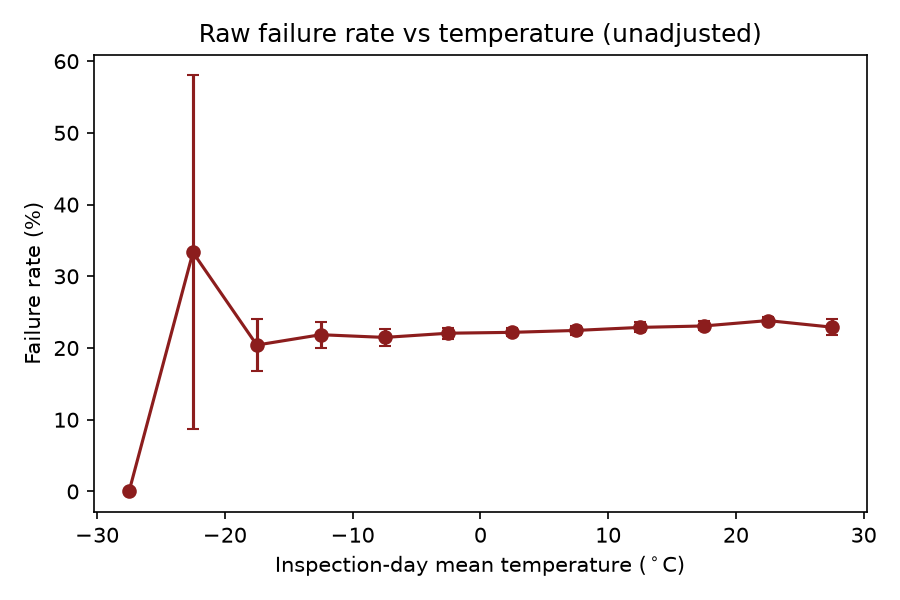
\includegraphics[width=0.62\linewidth]{fig2_raw_gradient.png}
\caption{Unadjusted failure rate by inspection-day temperature. The positive raw gradient
motivates---but does not survive---the within-establishment design.}
\label{fig:raw}
\end{figure}

\begin{figure}[H]\centering
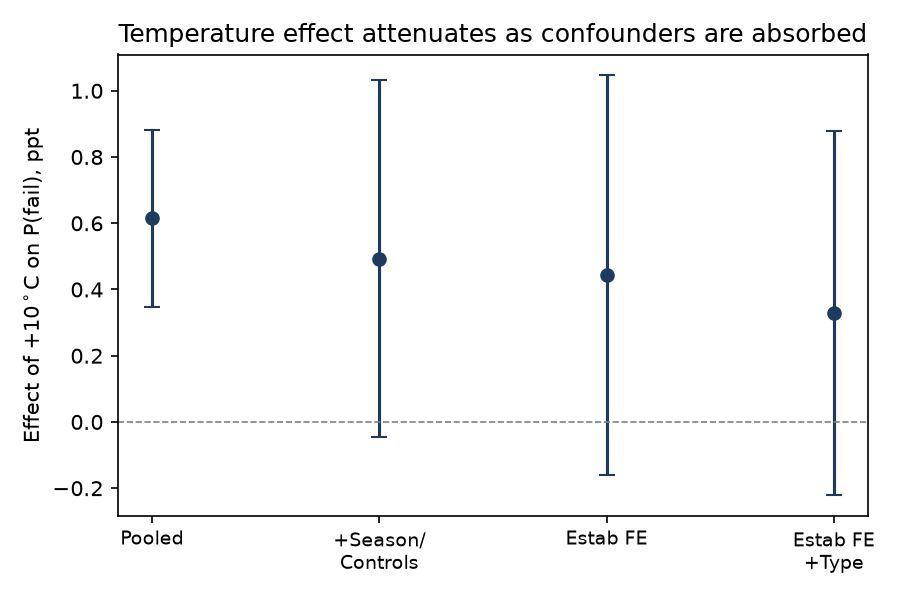
\includegraphics[width=0.62\linewidth]{fig1_attenuation.png}
\caption{The temperature coefficient (effect of $+10^\circ$C on the probability of failure,
in percentage points, with 95\% confidence intervals) attenuates toward zero as
establishment and seasonal fixed effects are absorbed.}
\label{fig:atten}
\end{figure}

\paragraph{Why the raw gradient is biased.}
The attenuation is driven by confounding, not by losing signal. A placebo that randomly
reassigns each inspection another day's weather yields 0.158~ppt ($p=0.22$), and replacing
month fixed effects with a cubic day-of-year polynomial yields 0.166~ppt ($p=0.54$)---both
null. The mechanism is compositional: inspection-day temperature does not predict the daily
\emph{volume} of inspections ($p=0.76$), but it strongly predicts their \emph{mix}, raising
the complaint-inspection share by 0.0148 per $+10^\circ$C and lowering the canvass share by
0.0256 (both $p<0.01$). Because complaint-driven visits fail more often, warmer-day
cross-sections look worse for reasons unrelated to food safety. This is precisely why
inspection type is a mediator and is excluded from the preferred design.

\section{Robustness}
Table~\ref{tab:robust} reports thirteen alternative specifications. The temperature
coefficient is positive in 92.3\% of them but significant at the .10 level in only 15.4\%;
the smallest $p$-value is 0.0312, which is 0.4056 after a Bonferroni correction, and 0.65
false positives are expected by chance at $\alpha=0.05$ across the thirteen tests.

Table~\ref{tab:inference} addresses inference and heterogeneity. Because weather is
autocorrelated across adjacent days, we re-cluster at the week and month level: the
preferred null is unchanged ($p=0.2236$ and $p=0.2392$). The two subsamples that look
significant under date clustering---routine canvasses and high-risk establishments---lose
significance under coarser clustering (canvass $p$ rises from 0.0312 to 0.0688, with a
wild-cluster bootstrap $p$ of 0.082; high-risk from 0.0612 to 0.1025). Restricting to
scheduled (non-complaint) inspections, which removes the endogenous timing of complaint
visits, gives 0.674~ppt ($p=0.0526$ by date, and $p=0.0959$/$0.1006$ under week/month
clustering)---borderline but not significant, and weaker under the design's preferred
inference.

\begin{table}[H]\centering
\caption{Robustness of the temperature coefficient across specifications}
\label{tab:robust}
\begin{tabular}{lcccc}
\hline\hline
Specification & $\hat\beta$ (ppt/10$^\circ$C) & SE & p & N \\
\hline
Primary (Estab+Month+Year+Type FE) & 0.329 & (0.280) & 0.240 & 116,466 \\
Cluster by establishment & 0.329 & (0.291) & 0.259 & 116,466 \\
Cluster by ZIP & 0.329 & (0.307) & 0.284 & 116,466 \\
Use daily MAX temp & 0.201 & (0.234) & 0.392 & 116,466 \\
Use apparent temp & 0.332 & (0.233) & 0.154 & 116,466 \\
Drop Type FE (Estab+Month+Year) & 0.443 & (0.308) & 0.151 & 116,466 \\
Add ZIP FE & 0.330 & (0.280) & 0.238 & 116,462 \\
Canvass inspections only & 0.853** & (0.396) & 0.031 & 57,636 \\
Restaurants only & 0.472 & (0.329) & 0.152 & 79,782 \\
Risk 1 (high) only & 0.575* & (0.307) & 0.061 & 92,828 \\
Pre-2020 only & 1.145 & (0.902) & 0.204 & 22,674 \\
2020+ only & -0.084 & (0.313) & 0.789 & 93,792 \\
Trim temp 1/99 pct & 0.464 & (0.291) & 0.111 & 114,272 \\
\hline
\multicolumn{5}{p{0.92\linewidth}}{\footnotesize Sign/significance agreement: 12/13 (92\%) positive; 2/13 (15\%) significant at .10; 2/13 (15\%) positive \emph{and} significant. The smallest p is 0.031 (Bonferroni-adjusted 0.406); 0.65 false positives are expected at $\alpha$=.05 across 13 tests. SE clustered by date unless noted. *** p$<$.01, ** p$<$.05, * p$<$.1.}\\
\end{tabular}
\end{table}

\begin{table}[H]\centering
\caption{Inference, contested subsamples, secondary outcome, and heterogeneity}
\label{tab:inference}
\begin{tabular}{lccc}
\hline\hline
\multicolumn{4}{l}{\emph{Panel A. Primary effect under coarser clustering (weather is autocorrelated)}}\\
Clustering $\rightarrow$ & Date & ISO-week & Year-month \\
 & (G=1969) & (G=415) & (G=96) \\
\hline
Primary (Estab+M+Y), full sample & 0.443 (0.151) & 0.443 (0.224) & 0.443 (0.239) \\
Scheduled (non-complaint) only & 0.674* (0.053) & 0.674* (0.096) & 0.674 (0.101) \\
\hline
\multicolumn{4}{l}{\emph{Panel B. Post hoc ``significant'' subsamples lose significance under correct inference}}\\
Canvass-only & 0.853** (0.031) & 0.853* (0.051) & 0.853* (0.069) \\
Risk 1 (high) only & 0.575* (0.061) & 0.575 (0.102) & 0.575 (0.102) \\
Canvass-only wild-cluster bootstrap p (month) & \multicolumn{3}{c}{0.082} \\
\hline
\multicolumn{4}{l}{\emph{Panel C. Secondary outcome: within-establishment violation count (NOT robust)}}\\
asinh(violations), no-Type FE & 0.017** (0.011) & 0.017** (0.032) & 0.017* (0.051) \\
violations (level), no-Type FE & 0.062** (0.022) & 0.062* (0.057) & 0.062* (0.083) \\
\multicolumn{4}{l}{\footnotesize \quad Count-family multiplicity: 12 tests, min p=0.007, Bonferroni=0.084 ($>$.05).}\\
\hline
\multicolumn{4}{l}{\emph{Panel D. Heterogeneity (H4, fail outcome): significant in baseline but NOT robust}}\\
$\times$ Restaurant$^\dagger$ (vs other facility) & 0.863*** (0.004) & 0.863*** (0.005) & 0.863** (0.014) \\
$\times$ Risk~1 (vs lower risk) & -0.176 (0.585) & -0.176 (0.604) & -0.176 (0.595) \\
\multicolumn{4}{l}{\footnotesize $^\dagger$Pre-registered leave-one-facility-out check FAILS: restaurant coef ranges 0.43--0.86 ppt, max p=0.171 (n.s.\ when Schools excluded). Stars notwithstanding, demoted to non-robust.}\\
\hline\hline
\multicolumn{4}{p{0.92\linewidth}}{\footnotesize Cells: coefficient with significance stars and (p-value). Panel A dep.\ var.\ \emph{fail}; B \emph{fail}; C as labeled (asinh / level of violation count); D interaction terms, dep.\ var.\ \emph{fail}. Panel A/B/D coefficients in percentage points. Coarser clusters guard against serial correlation in weather across adjacent days. *** p$<$.01, ** p$<$.05, * p$<$.1.}\\
\end{tabular}
\end{table}

\paragraph{Heterogeneity (pre-registered, demoted).}
A temperature-by-restaurant interaction is significant in the baseline (0.863~ppt,
$p=0.0037$) and survives coarse clustering. However, it \emph{fails} its pre-registered
must-pass diagnostic: leaving out one facility type at a time moves the coefficient between
0.43 and 0.863~ppt, with a maximum $p$-value of 0.1711---it becomes insignificant once
schools are removed from the comparison group. We therefore report it as a non-robust,
exploratory pattern rather than a finding. The risk-class interaction is null ($-0.176$~ppt,
$p=0.59$).

\paragraph{Secondary outcome.}
Within-establishment models of the citation count are positive but not robust: across the
family of count specifications the smallest $p$-value is 0.007, which exceeds 0.05 after
multiple-testing adjustment, and the count is itself mechanically tied to the failure
outcome. We do not treat it as corroborating evidence.

\section{Limitations}
Three limitations bound the interpretation. First, there is an identification ceiling:
because weather is constant within a calendar day, establishment-by-day fixed effects are
infeasible, so we cannot net out arbitrary correlated daily shocks; identification rests on
weather being exogenous within establishment and season. Second, the preferred estimate is a
reduced-form total effect that bundles any food-safety channel with temperature-driven
inspection selection; the scheduled-only subsample isolates the non-selection channel and is
also null. Third, the null is a \emph{bounded} null: it rules out average effects larger than
about 1.189~ppt per $+10^\circ$C (5.22\% of the base rate) but is underpowered against
modest effects, and weather is observed only at the daily citywide level. Results pertain to
Chicago over 2018--2026 and should not be extrapolated to other regimes.

\section{Conclusion}
Across a large administrative panel, the weather on inspection day has no robust effect on
whether a Chicago food establishment fails inspection. A plausible, mechanism-backed
cross-sectional correlation is fully explained by seasonal confounding and by
temperature-driven shifts in the composition of inspections. The episode is a concrete
reminder that within-unit variation, serially-robust inference, multiple-testing discipline,
and honest reporting of failed diagnostics can overturn an apparently significant headline.

\end{document}
